\section{Date: 2026-08-22}
\noindent \textbf{Series ID: EMISSCO2VDFCCBA} 

\noindent This series is titled Distillate Fuel Commercial Sector Carbon Dioxide Emissions and has a frequency of Annual. The units are Million Metric Tons CO2 and the seasonal adjustment is Not Seasonally Adjusted.The observation start date is 1973-01-01 and the observation end date is 2024-01-01.The popularity of this series is 1. \\ 

\noindent \textbf{Series ID: DDISCRT} 

\noindent This series is titled Discount Rate (DISCONTINUED) and has a frequency of Daily, 7-Day. The units are Percent and the seasonal adjustment is Not Seasonally Adjusted.The observation start date is 1955-01-03 and the observation end date is 2003-01-08.The popularity of this series is 8. \\ 

\subsection{Raw Regression}
\noindent Regresses the two series against each other directly. A significant result here can come just as easily from both series sharing a long-run trend as from any real relationship.

\begin{center}
\begin{tabular}{lclc}
\toprule
\textbf{Dep. Variable:}               & value\_fred\_DDISCRT & \textbf{  R-squared:         } &     0.029   \\
\textbf{Model:}                       &         OLS          & \textbf{  Adj. R-squared:    } &    -0.004   \\
\textbf{Method:}                      &    Least Squares     & \textbf{  F-statistic:       } &    0.8666   \\
\textbf{Date:}                        &   Sat, 22 Aug 2026   & \textbf{  Prob (F-statistic):} &    0.360    \\
\textbf{Time:}                        &       12:14:45       & \textbf{  Log-Likelihood:    } &   -75.337   \\
\textbf{No. Observations:}            &            31        & \textbf{  AIC:               } &     154.7   \\
\textbf{Df Residuals:}                &            29        & \textbf{  BIC:               } &     157.5   \\
\textbf{Df Model:}                    &             1        & \textbf{                     } &             \\
\textbf{Covariance Type:}             &      nonrobust       & \textbf{                     } &             \\
\bottomrule
\end{tabular}
\begin{tabular}{lcccccc}
                                      & \textbf{coef} & \textbf{std err} & \textbf{t} & \textbf{P$> |$t$|$} & \textbf{[0.025} & \textbf{0.975]}  \\
\midrule
\textbf{const}                        &       3.1251  &        3.421     &     0.913  &         0.369        &       -3.872    &       10.122     \\
\textbf{value\_fred\_EMISSCO2VDFCCBA} &       0.0775  &        0.083     &     0.931  &         0.360        &       -0.093    &        0.248     \\
\bottomrule
\end{tabular}
\begin{tabular}{lclc}
\textbf{Omnibus:}       &  6.919 & \textbf{  Durbin-Watson:     } &    0.447  \\
\textbf{Prob(Omnibus):} &  0.031 & \textbf{  Jarque-Bera (JB):  } &    5.197  \\
\textbf{Skew:}          &  0.866 & \textbf{  Prob(JB):          } &   0.0744  \\
\textbf{Kurtosis:}      &  4.012 & \textbf{  Cond. No.          } &     275.  \\
\bottomrule
\end{tabular}
%\caption{OLS Regression Results}
\end{center}

Notes: \newline
 [1] Standard Errors assume that the covariance matrix of the errors is correctly specified.

\begin{figure}
\centering
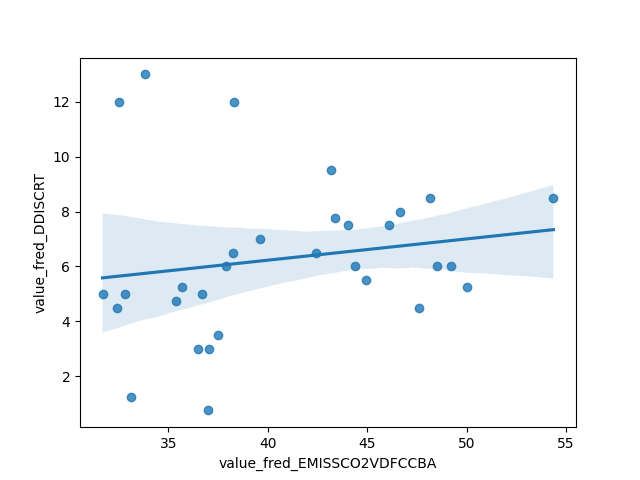
\includegraphics[scale = 0.9]{plots/plot_2026-08-22.png}
\caption{Raw Regression Plot for 2026-08-22}
\end{figure}
\newpage
\subsection{Detrended Regression}
\noindent Regresses the residuals of each series after removing its own linear time trend, so a shared trend can no longer drive the result on its own. A relationship that stays significant here is better evidence of a genuine link between the two series.

\begin{center}
\begin{tabular}{lclc}
\toprule
\textbf{Dep. Variable:}                          & value\_fred\_DDISCRT\_detrended & \textbf{  R-squared:         } &     0.138   \\
\textbf{Model:}                                  &               OLS               & \textbf{  Adj. R-squared:    } &     0.108   \\
\textbf{Method:}                                 &          Least Squares          & \textbf{  F-statistic:       } &     4.641   \\
\textbf{Date:}                                   &         Sat, 22 Aug 2026        & \textbf{  Prob (F-statistic):} &   0.0397    \\
\textbf{Time:}                                   &             12:14:45            & \textbf{  Log-Likelihood:    } &   -66.912   \\
\textbf{No. Observations:}                       &                  31             & \textbf{  AIC:               } &     137.8   \\
\textbf{Df Residuals:}                           &                  29             & \textbf{  BIC:               } &     140.7   \\
\textbf{Df Model:}                               &                   1             & \textbf{                     } &             \\
\textbf{Covariance Type:}                        &            nonrobust            & \textbf{                     } &             \\
\bottomrule
\end{tabular}
\begin{tabular}{lcccccc}
                                                 & \textbf{coef} & \textbf{std err} & \textbf{t} & \textbf{P$> |$t$|$} & \textbf{[0.025} & \textbf{0.975]}  \\
\midrule
\textbf{const}                                   &    1.604e-14  &        0.389     &  4.12e-14  &         1.000        &       -0.796    &        0.796     \\
\textbf{value\_fred\_EMISSCO2VDFCCBA\_detrended} &      -0.1840  &        0.085     &    -2.154  &         0.040        &       -0.359    &       -0.009     \\
\bottomrule
\end{tabular}
\begin{tabular}{lclc}
\textbf{Omnibus:}       &  1.468 & \textbf{  Durbin-Watson:     } &    0.556  \\
\textbf{Prob(Omnibus):} &  0.480 & \textbf{  Jarque-Bera (JB):  } &    0.984  \\
\textbf{Skew:}          & -0.000 & \textbf{  Prob(JB):          } &    0.612  \\
\textbf{Kurtosis:}      &  2.127 & \textbf{  Cond. No.          } &     4.55  \\
\bottomrule
\end{tabular}
%\caption{OLS Regression Results}
\end{center}

Notes: \newline
 [1] Standard Errors assume that the covariance matrix of the errors is correctly specified.

\begin{figure}
\centering
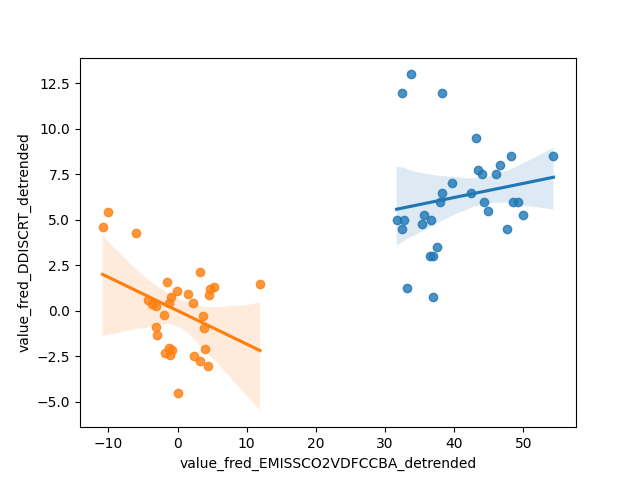
\includegraphics[scale = 0.9]{plots/plot_2026-08-22_detrended.png}
\caption{Detrended Regression Plot for 2026-08-22}
\end{figure}
\newpage
